% "{'classe':('PSI'),'chapitre':'chs_hs','type':('td'),'titre':'Système de dépose de poudre', 'source':'Concours Centrale Supélec - TSI 2016','comp':['B2-16',],'corrige':True}"
%\setchapterimage{bandeau}
\chapter*{TD \arabic{cptTD} :\\ 
Système de dépose de poudre -- \ifprof Corrigé \else Sujet \fi}
\addcontentsline{toc}{section}{TD \arabic{cptTD} : Système de dépose de poudre -- \ifprof Corrigé \else Sujet \fi}

\iflivret \stepcounter{cptTD} \else
\ifprof  \stepcounter{cptTD} \else \fi
\fi

\setcounter{question}{0}
\marginnote{Concours Centrale Supélec -- TSI 2016.}
\marginnote{
\UPSTIcompetence[2]{B2-16}
}

\begin{marginfigure}
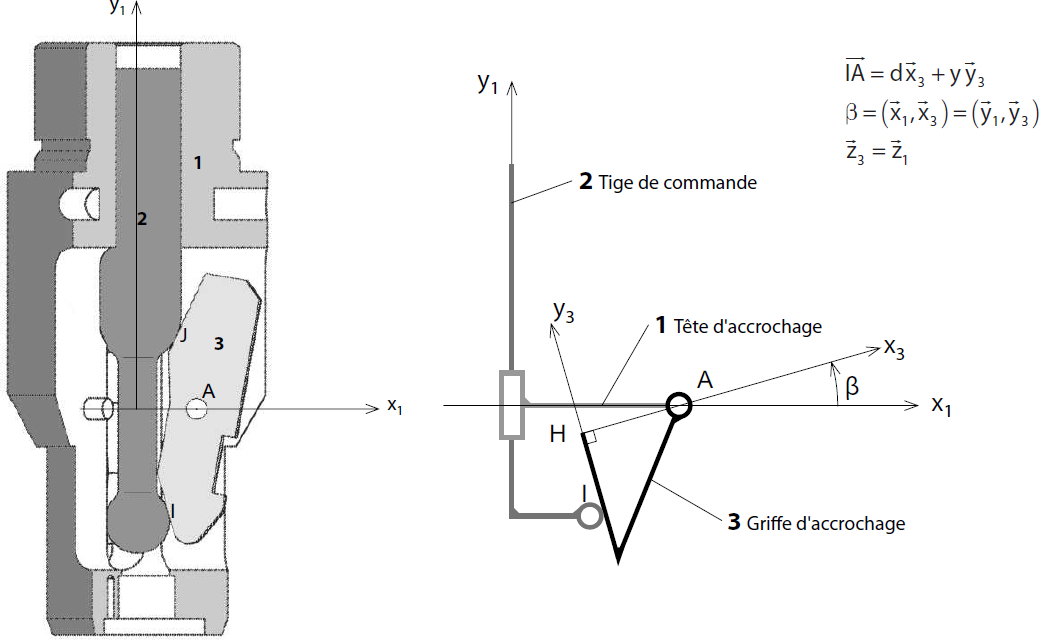
\includegraphics[width=\linewidth]{fig_01}
\end{marginfigure}


\section*{Mise en situation}
\ifprof
\else
On s'intéresse à un système permettant de créer des motifs sur de la poudre de maquillage compactée. Le poste de pulvérisation est en partie constitué d'un robot cartésien 3 axes permettant de déplacer des godets de poudre compactée (grâce à un préhenseur) en dessous de la buse de pulvérisation. 

\begin{center}
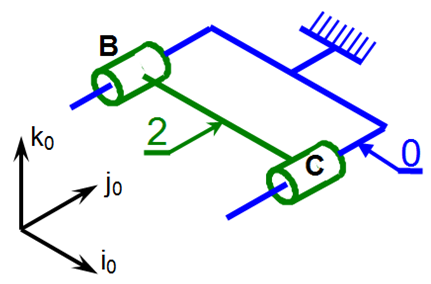
\includegraphics[width=.4\linewidth]{fig_02}
\end{center}

\fi

\begin{obj}
L’objectif de cette partie est de proposer un modèle du mécanisme constituant le déplacement de l’axe $\vect{x}$ et de justifier certains choix technologiques.
\end{obj}

\ifprof
\else
Le préhenseur repose sur des plaques support qui le lient en liaison encastrement au bâti. Les rails
guidant le préhenseur suivant l’axe $\vect{x}$ supportent les autres rails guidant les déplacement du préhenseur suivant les axes $\vect{y}$ et $\vect{z}$.

Le guidage est réalisé par deux axes munis de patins à billes.

\begin{marginfigure}
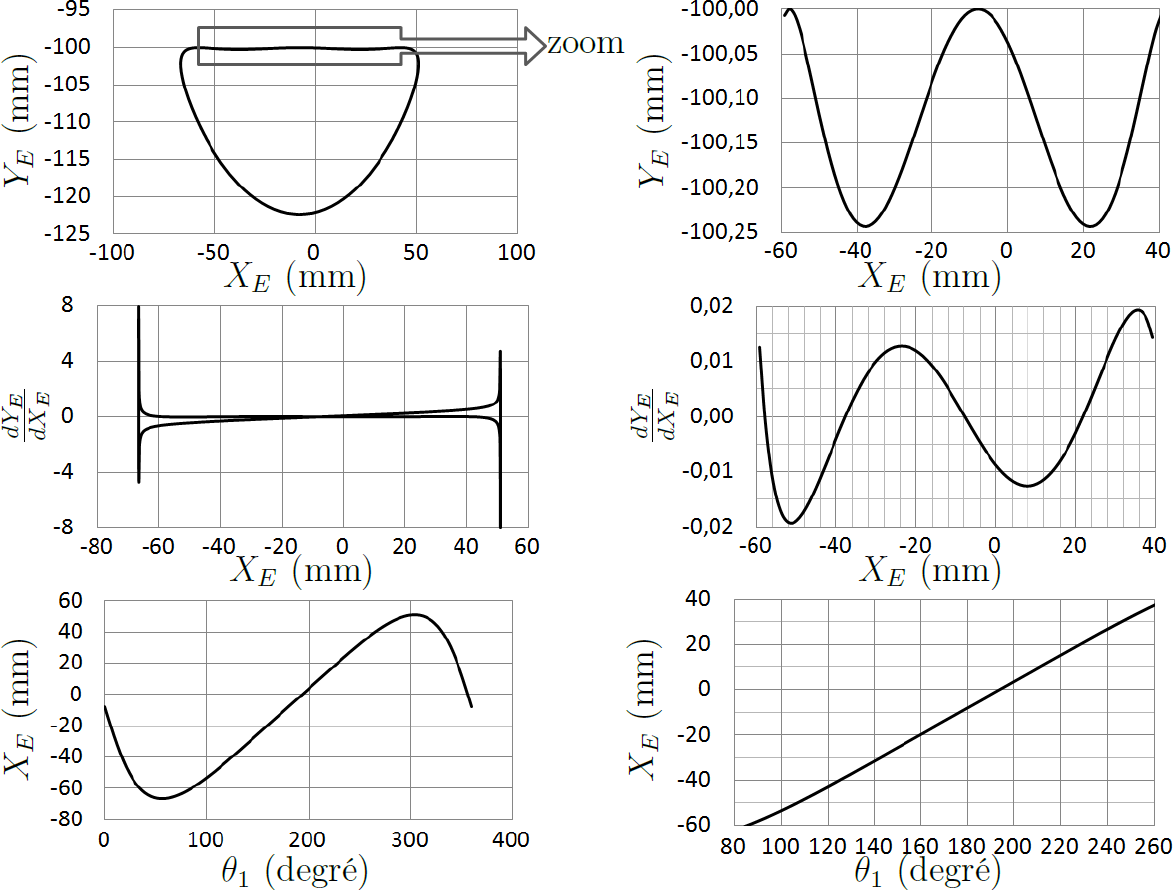
\includegraphics[width=\linewidth]{fig_03}
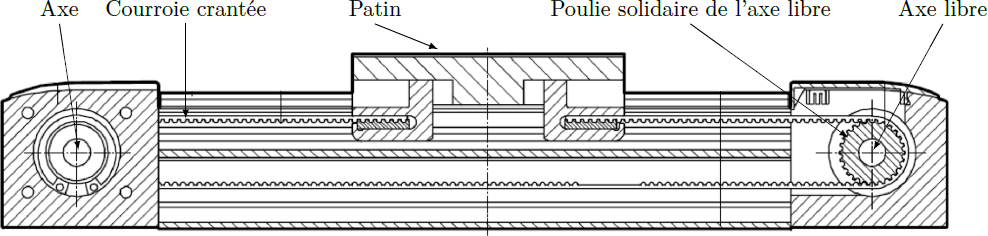
\includegraphics[width=\linewidth]{fig_04}
\end{marginfigure}

Le moteur actionnant l’axe $\vect{x}$ est lié à un réducteur qui entraîne deux ensembles poulies-courroies. Les poulies motrices sont guidées chacune par deux roulements à billes. Les deux poulies motrices sont liées par un arbre de transmission (Arbre 1). La
figure suivante représente le schéma cinématique de l’ensemble.

\begin{marginfigure}
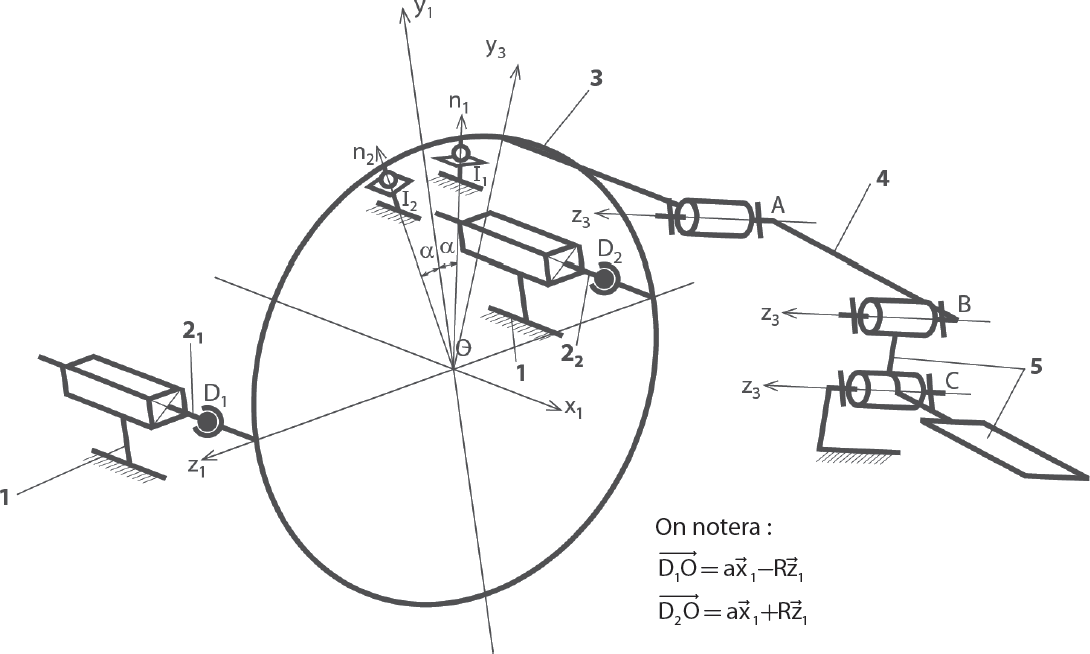
\includegraphics[width=\linewidth]{fig_05}
\end{marginfigure}
\fi


\section*{Travail demandé}

\ifprof
\else
La courroie étant un élément déformable, on n’en tiendra pas compte dans l’étude suivante.
\fi

\question{Déterminer le degré d’hyperstatisme de la liaison entre les solides 0 et 1.}
\ifprof
\begin{marginfigure}
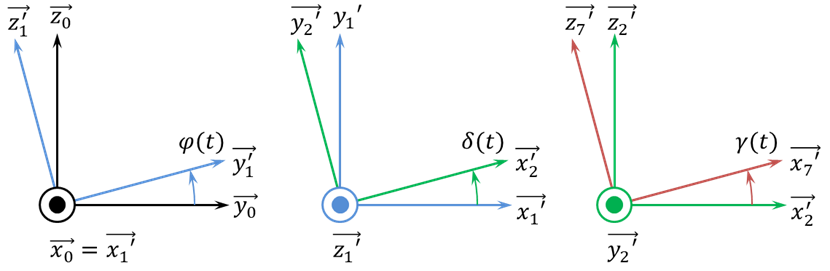
\includegraphics[width=\linewidth]{cor_01}
\end{marginfigure}

\begin{corrige} ~\\



\textbf{Méthode cinématique :}
\begin{itemize}
\item mobilité utile : $m_u=1$;
\item mobilité interne : $m_i=0$;
\item nombre de cycles : $\gamma = 1$;
\item nombre d'équations cinématiques : $E_c=6\gamma = 6$;
\item nombres d'inconnues cinématiques : $I_c=2\cdot 1=2$.
\end{itemize}
Au final : $h=m-I_c+E_c=1-2+6=5$.

\textbf{Méthode statique}
\begin{itemize}
\item mobilité utile : $m_u=1$;
\item mobilité interne : $m_i=0$;
\item nombre d'équations cinématiques : $E_s=6(p-1)=6(2-1)= 6$;
\item nombres d'inconnues cinématiques : $I_s=2\cdot 5 = 10$.
\end{itemize}
Au final : $h=m-E_s+I_s=1-6+10=5$.

\end{corrige}
\else
\fi

\ifprof
\else
Pour lever l’hyperstatisme de cette liaison, le constructeur a mis en place deux soufflets métalliques en les implantant de part et d’autre de l’arbre de transmission (figure suivante).

\begin{marginfigure}
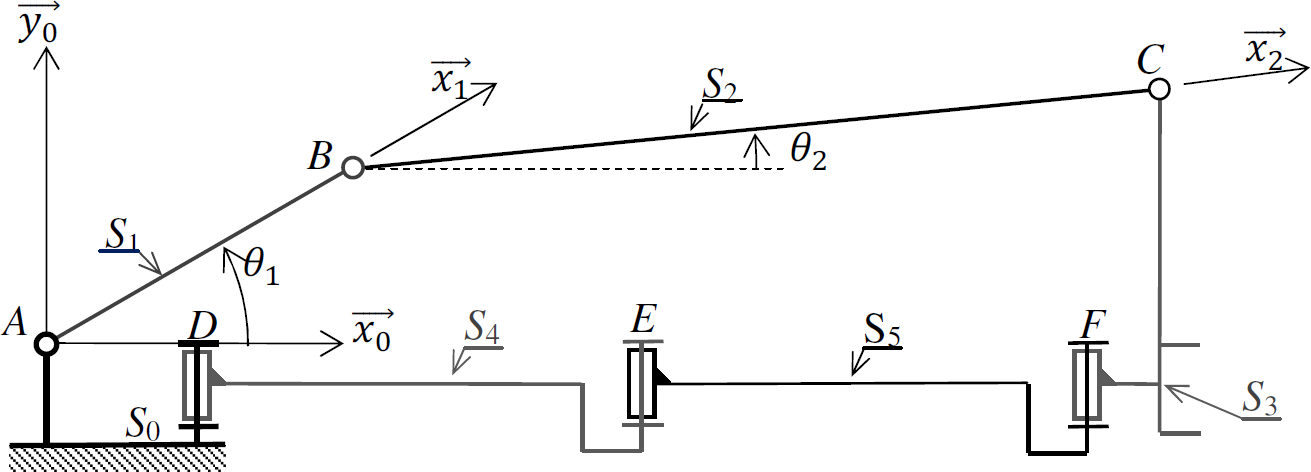
\includegraphics[width=\linewidth]{fig_06}
\end{marginfigure}

Un soufflet métallique est un joint d’accouplement autorisant des défauts d’alignement radiaux, axiaux et angulaires. Ainsi, pour un soufflet liant deux solides $S_1$ et $S_2$ positionné en un point $P$ et dont l’axe du soufflet est $\axe{P}{u}$ :
\begin{itemize}
\item le torseur statique transmissible est de la forme $\torseurstat{T}{S_1}{S_2}=\torseurcol{0}{0}{0}{L_{12}}{0}{0}{P,\base{u}{v}{w}}$;
\item le torseur cinématique du mouvement de $S_1$ par rapport à $S_2$ est de la forme $\torseurcin{V}{S_1}{S_2}=\torseurcol{0}{q_{12}}{r_{12}}{v_{x12}}{v_{y12}}{v_{z12}}{P,\base{u}{v}{w}}$.
\end{itemize}


L’introduction des deux soufflets métalliques impose de décomposer l’arbre 1 de la question 1 en 3 solides distincts $1_A$, $1_B$ et $1_C$ , le solide $1_B$ étant lié aux deux solides $1_A$ et $1_C$ par les deux soufflets métalliques.

\fi


\question{Tracer le nouveau graphe de liaisons en tenant compte de l’introduction des deux soufflets métalliques.}
\ifprof
\begin{corrige} ~\\

\begin{center}
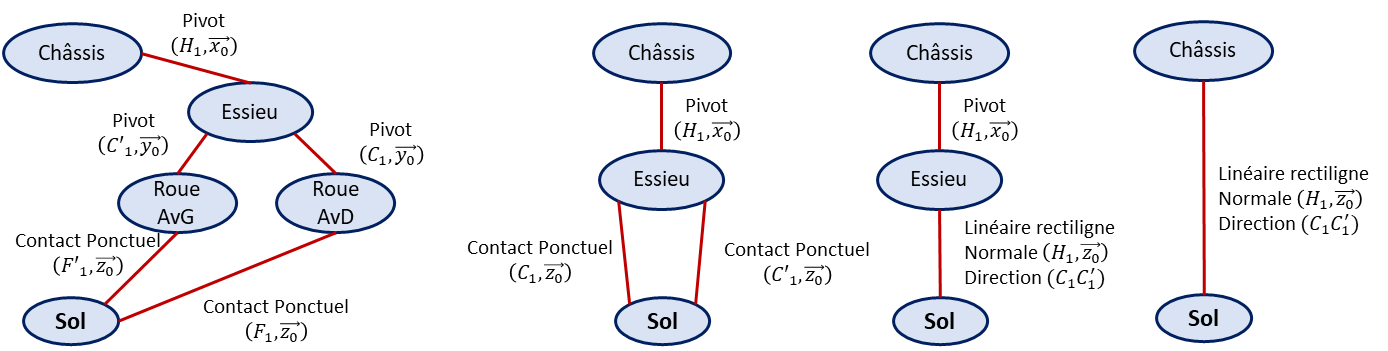
\includegraphics[width=7cm]{cor_02}
\end{center}

\end{corrige}
\else
\fi


\question{Déterminer en le justifiant le degré de mobilité du mécanisme ainsi modélisé en question précédente.}
\ifprof
\begin{corrige} ~\\
En réalisant une fermeture cinématique, on a $\torseurcin{V}{1_a}{0}+\torseurcin{V}{1_b}{1_a}+\torseurcin{V}{1_c}{1_b}=\torseurcin{V}{1_c}{0}$. 
Les torseurs étant considérés écrits au même point $P$, on a : 
$$
\left\{ 
\begin{array}{l}
p_{ba}+p_{cb}=0 \\
q_{ba}+q_{cb}=0 \\
r_{a0}=r_{c0}\\
\end{array}
\right. 
\quad
\left\{ 
\begin{array}{l}
v_{xba} + v_{xcb}=0\\
v_{yba} + v_{ycb}=0\\
v_{zba} + v_{zcb}=0\\
\end{array}
\right. .
$$
Il s'agit d'un système de rang 6 avec 12 inconnues. On a donc $m=I_c-r_c=12-6=6$.
\end{corrige}
\else
\fi


\question{En déduire le degré d’hyperstatisme du système avec ses deux soufflets métalliques.}
\ifprof
\begin{corrige} ~\\
On a $h=m-I_c+E_c = 6-12+6 = 0$.
\end{corrige}
\else
\fi

\ifprof
\else
\marginnote{
\begin{solution}
\begin{enumerate}
\item $h=5$.
\item ...
\item $m=6$.
\item $h=0$.
\item ...
\end{enumerate} 
\end{solution}}
\fi

\subsection*{Retour sur le cahier des charges}

\question{Conclure en justifiant l’utilisation des soufflets.}
\ifprof
\begin{corrige} ~\\
Le soufflet permet donc de rendre le système isostatique. Il est ainsi possible de monter le système sans avoir à imposer des contraintes géométriques sur le mécanisme. 
\end{corrige}
\else
\fi


